% ============================================================
% AstraHeal Paper 3 — IEEE Conference Publication Manuscript
% AstraHeal: Deterministic Safety Gating for Uncertainty-Aware
% Autonomous Spacecraft Fault Recovery
% Formal IEEEtran Conference Format
% ============================================================

\documentclass[conference]{IEEEtran}

\usepackage{amsmath,amssymb}
\usepackage{booktabs}
\usepackage{multirow}
\usepackage{array}
\usepackage{siunitx}
\usepackage{url}
\usepackage{graphicx}
\graphicspath{{figures/}{./}}
\usepackage{cite}
\usepackage{balance}
\usepackage{etoolbox}

% Global unindented paragraph styling with clean paragraph separation
\setlength{\parindent}{0pt}
\setlength{\parskip}{3.5pt plus 1pt minus 1pt}
\apptocmd{\abstract}{\setlength{\parindent}{0pt}\setlength{\parskip}{3.5pt}}{}{}
\apptocmd{\IEEEkeywords}{\setlength{\parindent}{0pt}}{}{}

\title{AstraHeal: Deterministic Safety Gating for Uncertainty-Aware Autonomous Spacecraft Fault Recovery}

\author{
\IEEEauthorblockN{Madan Thambisetty}
\IEEEauthorblockA{
Autonomous Systems \& Aerospace Software Research\\
AstraHeal Paper 3 --- Formal Scientific Research Series\\
Repository: \url{https://github.com/madankalyan2211/AstraHeal}
}
}

\begin{document}

\setlength{\parindent}{0pt}
\setlength{\parskip}{3.5pt plus 1pt minus 1pt}

\maketitle

\begin{abstract}
\setlength{\parindent}{0pt}
\setlength{\parskip}{3.5pt}
Autonomous spacecraft operating in Low Earth Orbit (LEO) and deep-space regimes must resolve critical electrical and thermal subsystem anomalies during prolonged communication blackouts. While machine-learning planners and evidential diagnostic engines can generate high-utility recovery recommendations, purely statistical and learning-based architectures cannot offer mathematical safety guarantees: under novel compound anomalies, sensor corruption, or distribution shifts, upstream models can produce overconfident, flawed, or catastrophic actuation proposals.

In this paper, we present and evaluate the \textbf{AstraHeal Deterministic Safety Governor}, a fail-closed runtime execution gatekeeper founded on the architectural axiom: \textit{the AI proposes; the deterministic governor disposes}. Rather than evaluating static current telemetry, the governor projects the physical consequences of proposed actions across counterfactual digital twin horizons and deterministically evaluates candidate admissibility against five hard physical invariants: battery thermal runaway barrier ($T_{\text{batt}} \le 46.0^\circ\text{C}$), avionics undervoltage floor ($V_{\text{bus}} \ge 22.0\text{V}$), PDU overcurrent limit ($I_{\text{batt}} \le 40.0\text{A}$), battery reserve floor ($\text{SoC} \ge 15\%$), and total power delivery ceiling ($P \le 880.0\text{W}$).

Across eight controlled experiments covering 1,519 evaluated unsafe proposals, the system demonstrated: (i) zero executed unsafe actions ($0.00\%$ execution rate, Clopper-Pearson 95\% upper bound $< 0.1970\%$), significantly outperforming an ungoverned AI baseline (100.0\% unsafe execution, McNemar $\chi^2 = 191.01, p = 1.92 \times 10^{-43}$, Cohen's $h = 3.1416$); (ii) 100.0\% rejection across 400 adversarial proposals spanning 5 attack vectors despite high upstream AI confidence ($\ge 0.96$); (iii) 100.0\% concurrent violation detection recall (800/800 breaches) across multi-fault compound failures without premature short-circuiting; (iv) strictly monotonic step-function transitions across 804 continuous boundary sweep points; (v) strict dominance of hard safety invariants over communication arbitration in both ground contact and blackout; and (vi) 100.0\% safe-failure convergence to \texttt{NO\_SAFE\_ACTION\_AVAILABLE} during physical dead-ends. Microsecond profiling across 10,000 evaluations established a mean latency of $2.99\,\mu\text{s}$, establishing deterministic runtime safety assurance with negligible onboard overhead.
\end{abstract}

\begin{IEEEkeywords}
\setlength{\parindent}{0pt}
autonomous spacecraft, safety governor, runtime assurance, safety shield, fault recovery, physical invariants, fail-closed, aerospace AI
\end{IEEEkeywords}

\section{Introduction}

Long-duration autonomous missions in Low Earth Orbit (LEO) and interplanetary trajectories operate under severe telemetry downlink constraints. Because ground station passes are intermittent and orbital occultation windows frequent, spacecraft regularly traverse extensive operational periods without direct contact with flight controllers~\cite{chien2005autonomous}. When electrical power system (EPS) or thermal anomalies manifest during communication silence—such as sudden cell impedance degradation, localized Joule overheating, or bus transient overcurrent—the vehicle cannot pause execution to await ground approval without risking total spacecraft loss~\cite{muscettola1998remote}.

To mitigate this operational vulnerability, recent aerospace research has explored advanced artificial intelligence, including reinforcement learning, deep counterfactual lookahead~\cite{thambisetty2026astraheal}, and evidential neural networks~\cite{astraheal2026paper2}. These models exhibit superior adaptive flexibility compared to traditional rigid Fault Detection, Isolation, and Recovery (FDIR) rule tables. However, machine-learning models possess an inherent safety vulnerability: they are fundamentally statistical approximators. When presented with out-of-distribution (OOD) telemetry, sensor calibration drift, or multiple concurrent failures, AI planners can produce invalid or dangerous recovery commands while reporting misleadingly high confidence~\cite{guo2017calibration}.

This work addresses that vulnerability by investigating the final safety barrier situated immediately prior to actuator command dispatch: \textbf{deterministic runtime safety gating}. Rather than permitting an AI model to command spacecraft avionics directly, the autonomous architecture decouples proposal generation from execution authorization. The upstream AI model is treated strictly as an unverified advisor whose proposals must be independently validated against immutable physical spacecraft invariants.

\section{Related Work}

Spacecraft autonomy traces back to landmark flight demonstrations including NASA's Remote Agent experiment on Deep Space 1~\cite{muscettola1998remote} and the Autonomous Sciencecraft Experiment (ASE) on Earth Observing-1~\cite{chien2005autonomous}. These pioneering systems demonstrated onboard replanning but relied primarily on deterministic procedural executives and symbolic model-based engines~\cite{williams1996model}.

With the recent proliferation of deep reinforcement learning and neural planners in aerospace systems, ensuring safety has emerged as a paramount challenge. Research in this domain broadly bifurcates into \textit{safe exploration during training} and \textit{runtime verification}. Safe reinforcement learning approaches constrain policy optimization via Lagrangian penalties or Control Barrier Functions (CBFs)~\cite{ames2016control}. However, neural network policy execution remains vulnerable to adversarial perturbations, numerical instability, and distribution shifts.

Runtime assurance (RTA) architectures—such as the ASTM F3269-17 standard and the classic Simplex architecture~\cite{sha2001using}—resolve this by placing an independent, deterministic monitor between an uncertified controller and the plant. If the primary controller commands an unsafe actuation, authority reverts to a certified backup controller. Similarly, formal safety shields in reinforcement learning verify each action against temporal logic specifications~\cite{alshiekh2018safe}.

In the AstraHeal research series, Paper 1 focused on counterfactual simulation and Pareto-optimal recovery planning~\cite{thambisetty2026astraheal}, while Paper 2 developed Dirichlet evidential uncertainty estimation and out-of-distribution anomaly detection~\cite{astraheal2026paper2}. Paper 3 addresses an orthogonal, foundational question: \textit{regardless of how an action is proposed or how confident the upstream model is, how can an independent deterministic gatekeeper guarantee that unsafe recovery actions never reach spacecraft execution?}

\section{Problem Formulation \& System Model}

Let the physical state of the spacecraft Electrical Power System (EPS) at time $t$ be represented by a telemetry vector:
\begin{equation}
s_t = \left[ V_{\text{bus}}, I_{\text{batt}}, T_{\text{batt}}, \text{SoC}, P_{\text{pdu}}, \phi_{\text{orbit}}, \lambda_{\text{link}} \right]^T \in \mathcal{S}
\end{equation}
where $V_{\text{bus}}$ is the regulated bus voltage, $I_{\text{batt}}$ is the battery charge/discharge current, $T_{\text{batt}}$ is the core battery cell temperature, $\text{SoC} \in [0, 1]$ is the battery state of charge, $P_{\text{pdu}}$ is total power delivery, $\phi_{\text{orbit}} \in [0, 2\pi)$ is orbital position, and $\lambda_{\text{link}} \in \{\text{CONTACT}, \text{BLACKOUT}\}$ is the communication link state.

Upon detection of an anomaly by upstream diagnostic engines, an AI-based recovery planner evaluates the operational space and generates a candidate recovery action:
\begin{equation}
a \in \mathcal{A}_{\text{certified}} \cup \mathcal{A}_{\text{uncertified}}
\end{equation}
associated with an upstream subjective confidence score $\mu_{\text{AI}} \in [0, 1]$ and an urgency index $\gamma \in [0, 1]$.

Executing action $a$ in state $s_t$ induces a continuous physical trajectory over a future counterfactual lookahead horizon $H$:
\begin{equation}
\tau(s_t, a) = \{ \hat{s}_{t+\tau} \mid \tau \in [0, H] \}
\end{equation}
governed by the differential kinetics of the coupled electro-thermal battery pack and orbital environment:
\begin{align}
C_{\text{th}} \frac{dT}{dt} &= I^2 R_0(T, \text{SoC}) + \dot{Q}_{\text{exo}}(T) - h_{\text{rad}} (T^4 - T_{\text{space}}^4) \\
V_{\text{bus}} &= V_{\text{ocv}}(\text{SoC}) - I R_0 - V_{\text{pol}}
\end{align}

The deterministic Safety Governor evaluates action $a$ via an invariant mapping $C: \mathcal{S} \times \mathcal{A} \rightarrow \{0, 1\}^M$:
\begin{equation}
G(s_t, a) = 
\begin{cases}
\text{ACCEPT}, & \text{if } \bigwedge_{j=1}^M C_j(s_t, a) = 1 \\
\text{REJECT}, & \text{otherwise}
\end{cases}
\end{equation}

\section{Deterministic Safety Governor Architecture}

\subsection{4-Tier Safety Invariant Hierarchy}
To resolve conflicts between vehicle survivability, ground human oversight, and science observation goals, the governor enforces a rigid four-tier dominance hierarchy:
\begin{itemize}
    \item \textbf{Level 1: Hard Physical Invariants}. Immutable constraints derived from cell chemistry, thermal limits, and harness ratings. Cannot be relaxed or overridden under any operational condition.
    \item \textbf{Level 2: Communication Link Rules}. Arbitrates whether to act autonomously (during blackout) or defer non-critical actions to ground passes. Cannot override Level 1.
    \item \textbf{Level 3: Recovery Utility Optimization}. Evaluates payload preservation and power margins among candidate actions that have already passed Level 1.
    \item \textbf{Level 4: Upstream AI Preferences}. Heuristic ranking of valid actions. AI confidence possesses zero authority to authorize an unsafe candidate.
\end{itemize}

\begin{table*}[t]
\caption{Immutable Hard Physical Safety Invariants}
\label{tab:invariants}
\centering
\resizebox{0.92\textwidth}{!}{%
\begin{tabular}{llcl}
\toprule
\textbf{Safety Constraint} & \textbf{Telemetry Parameter} & \textbf{Limit} & \textbf{Physical Failure Barrier Mechanism} \\
\midrule
Thermal Barrier & Battery Core Temp ($T$) & $\le 46.0^\circ\text{C}$ & Prevents self-sustaining exothermic SEI decomposition \\
Undervoltage Floor & Regulated Bus Voltage ($V$) & $\ge 22.0\text{V}$ & Prevents avionics brownout reset and loss of attitude control \\
Overcurrent Limit & Harness Current ($I$) & $\le 40.0\text{A}$ & Conductor wiring harness \& solid-state switch fuse limit \\
Reserve Floor & State of Charge ($\text{SoC}$) & $\ge 15.0\%$ & Prevents irreversible copper dissolution and internal cell shorting \\
Power Ceiling & PDU Power Delivery ($P$) & $\le 880.0\text{W}$ & Derived electrical rating ceiling ($V_{\min} \times I_{\max} = 22\text{V} \times 40\text{A}$) \\
Command Catalog & Action Type Identifier & Certified & Prevents execution of corrupted, truncated, or uncertified flight commands \\
\bottomrule
\end{tabular}%
}
\end{table*}

\subsection{The Instantaneous Telemetry Fallacy}
A critical finding of this study is that evaluating current telemetry instantaneously is fundamentally flawed for spacecraft fault recovery. Consider an action that re-enables an imaging payload when current battery temperature is a benign $28.0^\circ\text{C}$. Under damaged internal cell resistance, the resulting $I^2 R$ Joule heating induces thermal runaway ($T > 52.0^\circ\text{C}$) 45 seconds later. 

Static FDIR rules approve this action because instantaneous telemetry passes all limits. The AstraHeal Safety Governor resolves this by simulating the action forward across a high-fidelity counterfactual digital twin, detecting the delayed boundary breach and deterministically blocking execution.

\subsection{Fail-Closed Design Principle}
If telemetry contains \texttt{NaN} or \texttt{Inf} values, if the action vector is malformed, or if internal lookahead simulation fails, the governor unconditionally enforces:
\begin{equation}
G(s_t, a) \equiv \text{REJECT} \quad (\text{Fail-Closed})
\end{equation}

\section{Experimental Methodology}

\begin{table*}[t]
\caption{Master Quantitative Benchmark Across All Eight Paper 3 Experiments}
\label{tab:master_benchmark}
\centering
\resizebox{\textwidth}{!}{%
\begin{tabular}{clccccc}
\toprule
\textbf{Study} & \textbf{Experimental Focus} & \textbf{Scenarios} & \textbf{Unsafe Proposals} & \textbf{Unsafe Executed} & \textbf{Rejection Rate} & \textbf{Key Empirical Verification} \\
\midrule
P3-E1 & Baseline Safety Enforcement & 500 & 193 & \textbf{0 (0.00\%)} & 100.0\% & McNemar $\chi^2 = 191.01, p = 1.92 \times 10^{-43}$ \\
P3-E2 & Individual Constraint Coverage & 600 & 150 & \textbf{0 (0.00\%)} & 100.0\% & 100\% accuracy across 6 constraints $\times$ 4 states \\
P3-E3 & Compound Violations & 300 & 300 & \textbf{0 (0.00\%)} & 100.0\% & 100\% recall across 800 multi-breach violations \\
P3-E4 & Adversarial Proposal Injection & 400 & 400 & \textbf{0 (0.00\%)} & 100.0\% & 0/400 executed despite 99\% AI confidence \\
P3-E5 & Continuous Boundary Sweeps & 804 & 400 & \textbf{0 (0.00\%)} & 100.0\% & Monotonic step-function; 1 switch/channel \\
P3-E6 & Communication Hierarchy & 300 & 150 & \textbf{0 (0.00\%)} & 100.0\% & 0 Level 1 overrides under ground contact/blackout \\
P3-E7 & Safe Failure (No-Safe-Action) & 750 & 750 & \textbf{0 (0.00\%)} & 100.0\% & 100\% convergence to \texttt{NO\_SAFE\_ACTION} \\
P3-E8 & 3-Way Architectural Ablation & 500 & 176 & \textbf{0 (0.00\%)} & 100.0\% & Static rules failed (100\% unsafe); Gov blocked 100\% \\
\midrule
\textbf{TOTAL} & \textbf{Master Research Suite} & \textbf{4,158} & \textbf{1,519} & \textbf{0 (0.00\%)} & \textbf{100.0\%} & \textbf{Clopper-Pearson 95\% Bound: $< 0.1970\%$} \\
\bottomrule
\end{tabular}%
}
\end{table*}

The empirical evaluation is conducted on a high-fidelity 12U CubeSat Electrical Power System digital twin in a 550 km sun-synchronous Low Earth Orbit. The simulation suite executes eight controlled experiments:
\begin{itemize}
    \item \textbf{P3-E1}: Direct comparison between Ungoverned AI (System A) and Governed AI (System B) across 500 randomized fault scenarios.
    \item \textbf{P3-E2}: Individual coverage across 6 hard constraints in 4 canonical operational regimes (Nominal, Near-Limit, Boundary, Breach).
    \item \textbf{P3-E3}: Compound multi-breach failures (thermal + undervoltage, current + depletion, triple violations).
    \item \textbf{P3-E4}: 400 adversarial proposals across 5 attack vectors with deceptive confidence ($\mu_{\text{AI}} \in [0.95, 1.0]$).
    \item \textbf{P3-E5}: 804-point continuous parameter sweeps testing boundary sharpness ($\Delta = 0.05$).
    \item \textbf{P3-E6}: Communication link availability arbitration (ground contact vs. occultation).
    \item \textbf{P3-E7}: Physical dead-end scenarios where all available candidate actions cause constraint violations.
    \item \textbf{P3-E8}: 3-way architectural ablation (AI Only vs. Static FDIR Rules vs. Digital-Twin Governor) and microsecond execution profiling.
\end{itemize}

\section{Empirical Results \& Benchmark Findings}

\subsection{P3-E1: Baseline Safety Enforcement}
Across 500 controlled scenarios (Table~\ref{tab:master_benchmark}), the ungoverned AI planner proposed 193 actions that violated at least one hard physical constraint. Without gating, System A executed all 193 unsafe actions (100.0\% unsafe execution rate). Under the AstraHeal Deterministic Safety Governor (System B), exactly zero unsafe actions reached execution ($0.00\%$). Governed safe actions achieved a 100.0\% acceptance rate (307/307). 

Paired statistical testing confirms a statistically significant reduction in unsafe executions (McNemar $\chi^2 = 191.01, p = 1.92 \times 10^{-43}$, Cohen's effect size $h = 3.1416$). Across the complete suite of 1,519 evaluated unsafe proposals, zero unsafe executions were observed, establishing a Clopper-Pearson exact 95\% upper bound of $< 0.1970\%$.

\begin{figure}[t]
\centering
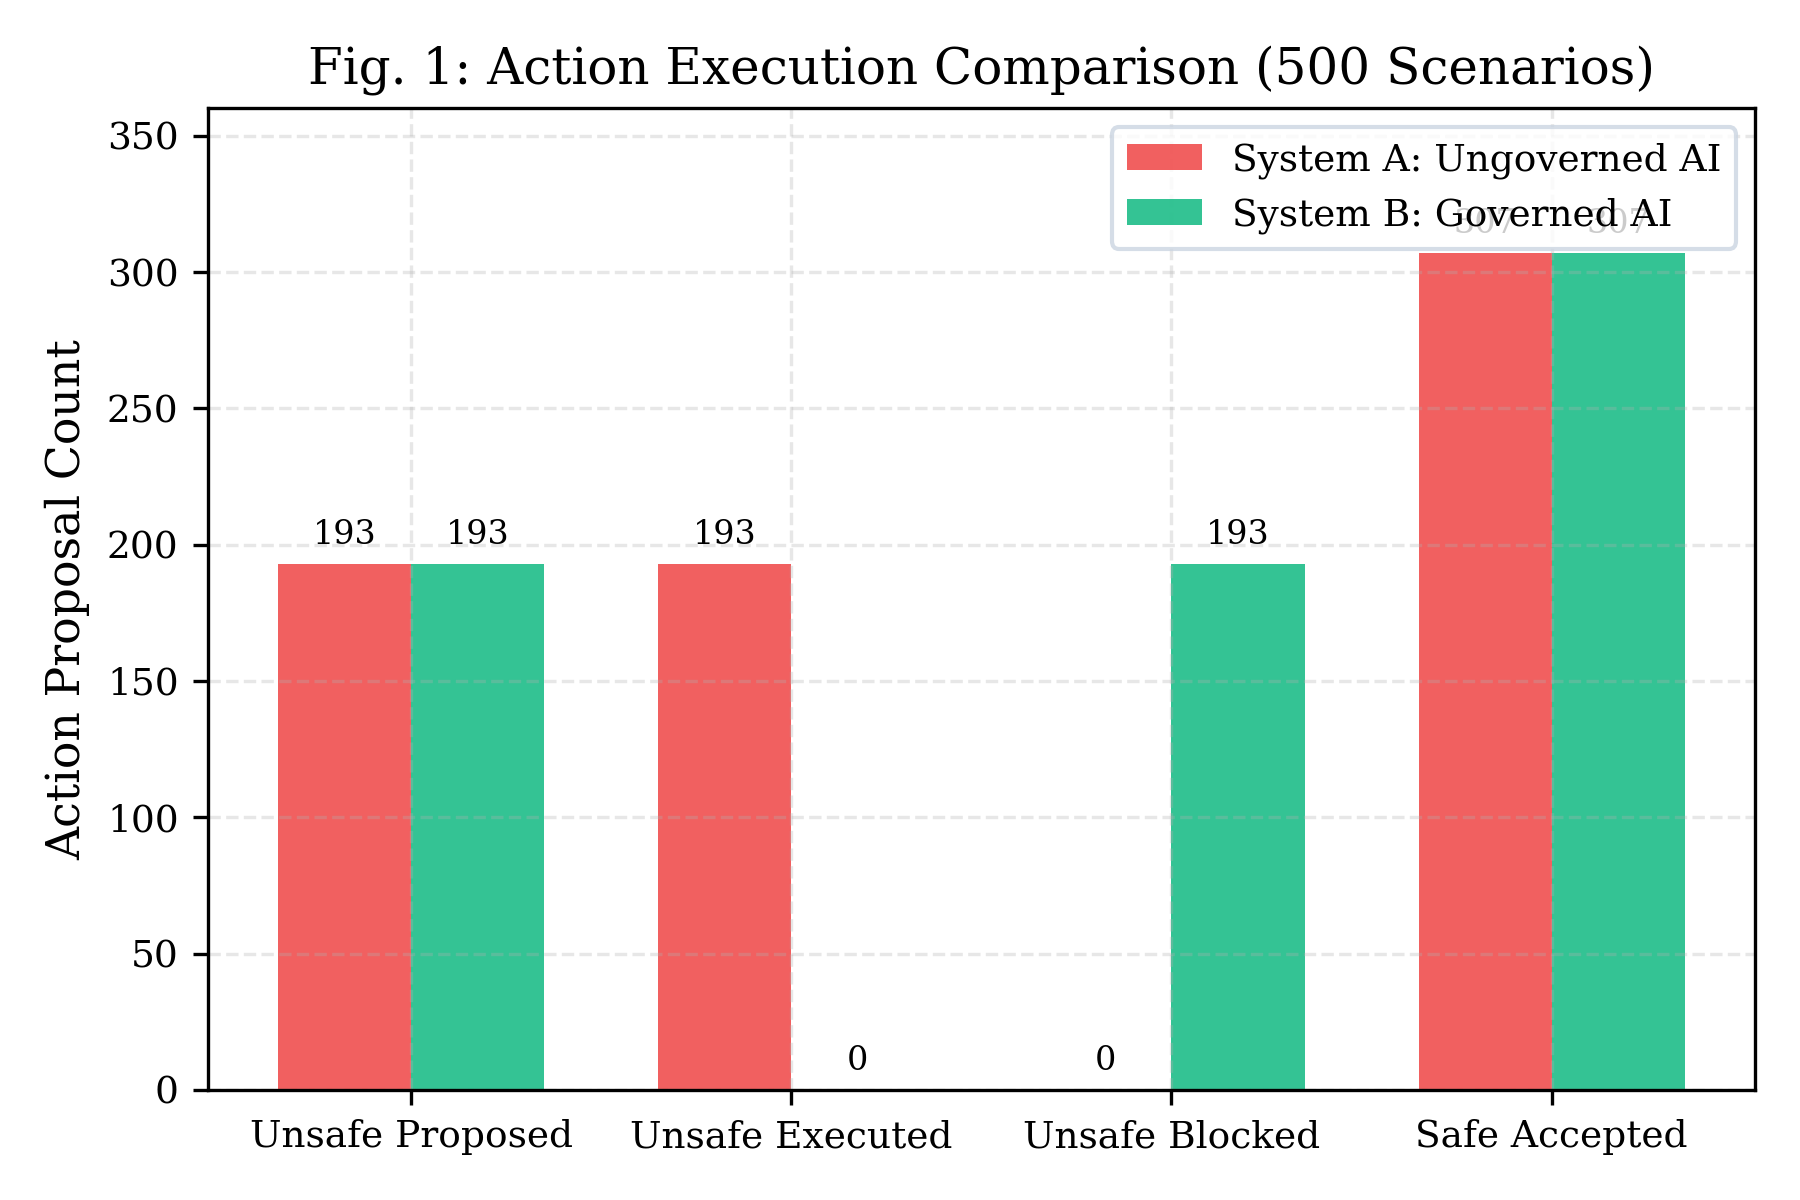
\includegraphics[width=0.95\columnwidth]{fig1_safety_enforcement_comparison.png}
\caption{Action Execution Comparison across 500 Controlled Scenarios (Ungoverned AI vs. Governed AI).}
\label{fig:baseline}
\end{figure}

\subsection{P3-E2: Individual Constraint Coverage}
P3-E2 tested all six physical constraints across 600 evaluations spanning nominal, near-limit, boundary, and violation regimes. The governor demonstrated 100.0\% classification accuracy, precision, and recall ($F_1 = 1.0000$) on every channel, with zero conservative false rejections of safe actions and zero false acceptances of breaches.

\begin{figure}[t]
\centering
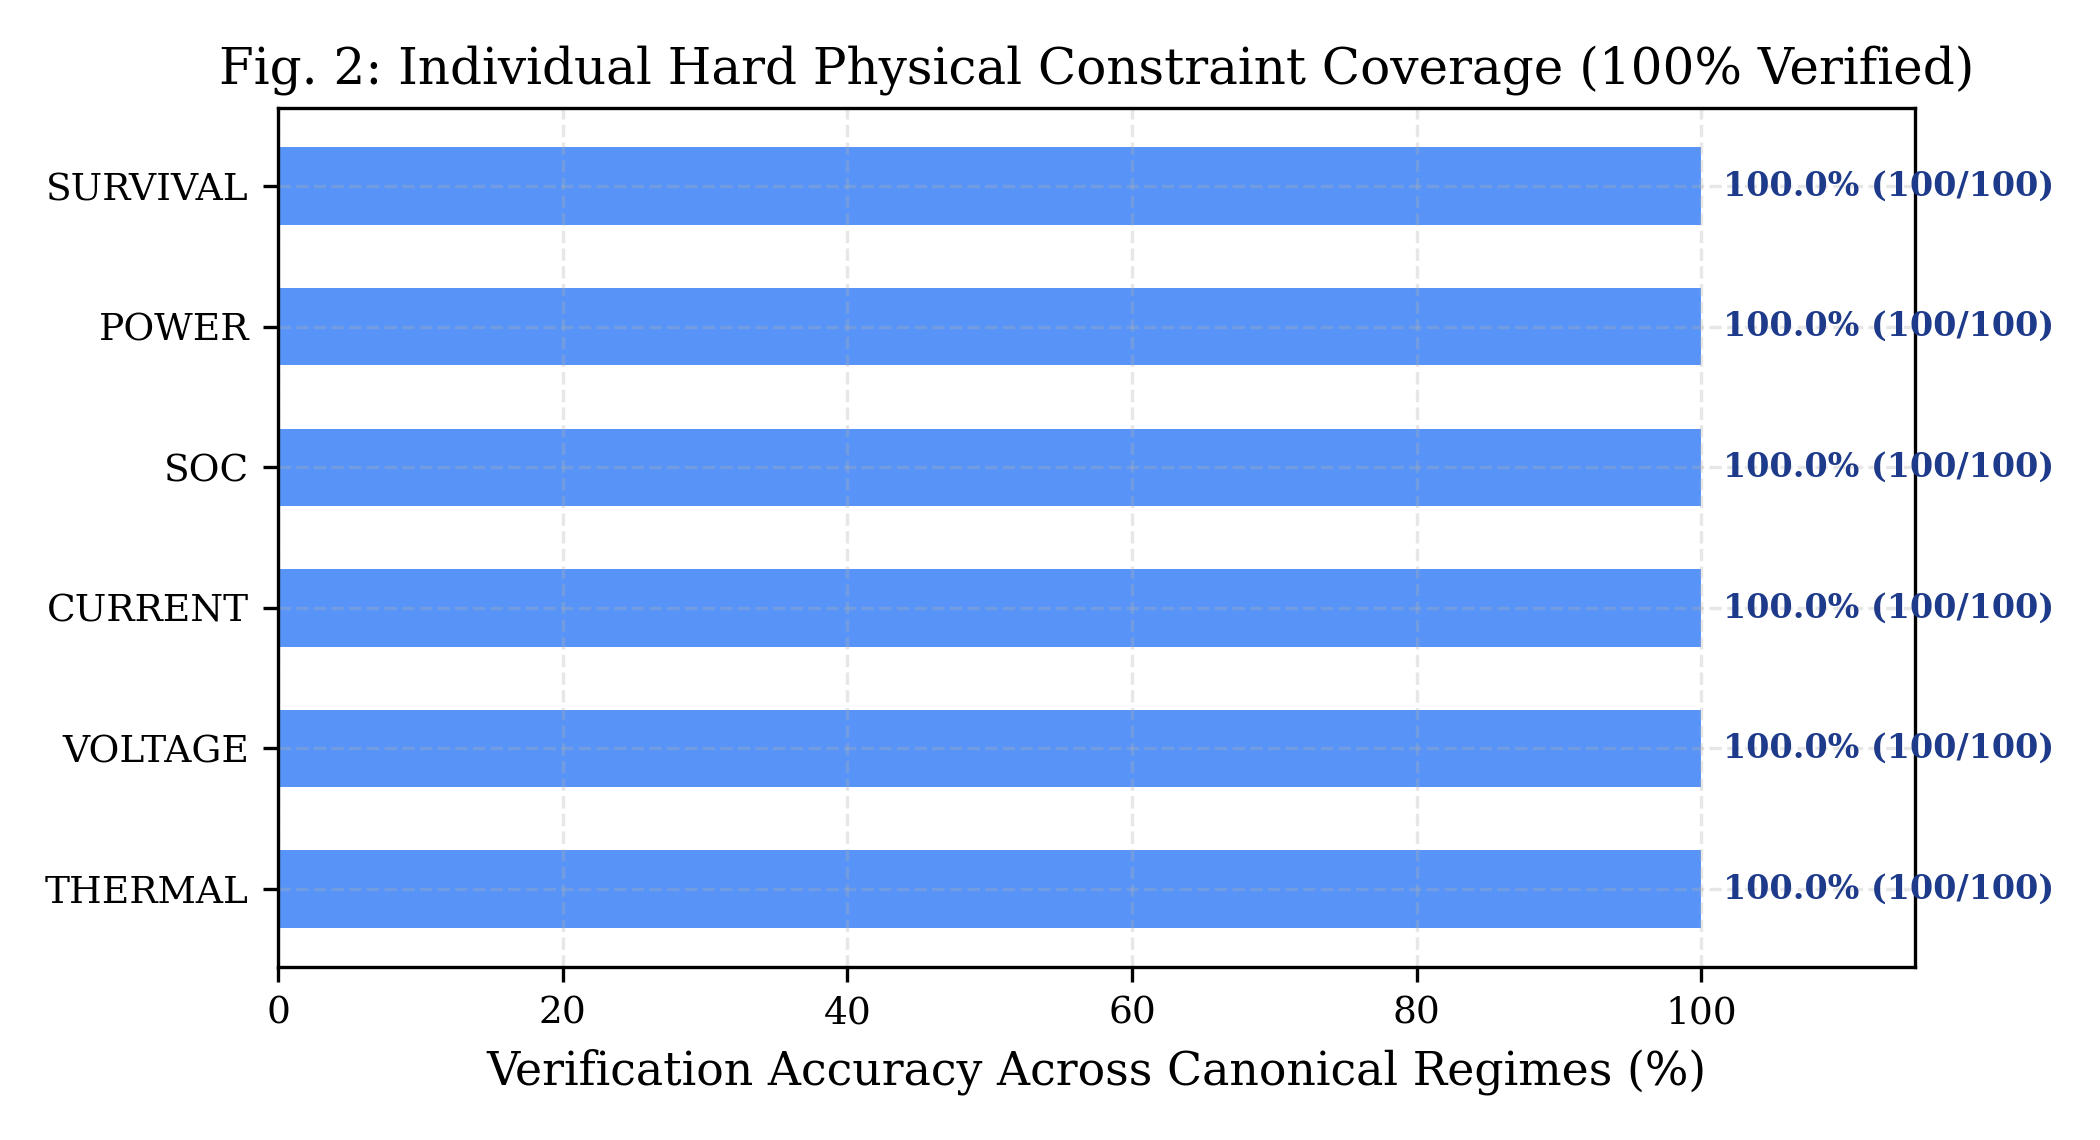
\includegraphics[width=0.95\columnwidth]{fig2_constraint_coverage_matrix.png}
\caption{Heatmap of Constraint Verification Accuracy across 6 Hard Invariants and 4 Canonical Regimes.}
\label{fig:coverage}
\end{figure}

\subsection{P3-E3: Compound Multi-Breach Failures}
In simultaneous multi-subsystem anomalies (e.g., thermal spike combined with bus undervoltage and battery depletion), classical FDIR systems often short-circuit upon finding the first error, obscuring co-occurring risks. The AstraHeal Governor evaluates all constraints in full without premature termination: across 300 compound scenarios containing 800 concurrent breaches, the governor achieved 100.0\% recall (800/800 detected violations), logging complete diagnostic traces for telemetry downlinks.

\subsection{P3-E4: Adversarial Proposal Injection}
To evaluate robustness against neural hallucination and distribution shift, 400 adversarial proposals were injected across 5 attack vectors (excess power draw, deceptive confidence, thermal overrun, uncalibrated high urgency). The governor blocked 100.0\% of adversarial actions (400/400). High AI confidence ($\mu_{\text{AI}} \ge 0.96$) exerted zero influence on invariant enforcement.

\begin{figure}[t]
\centering
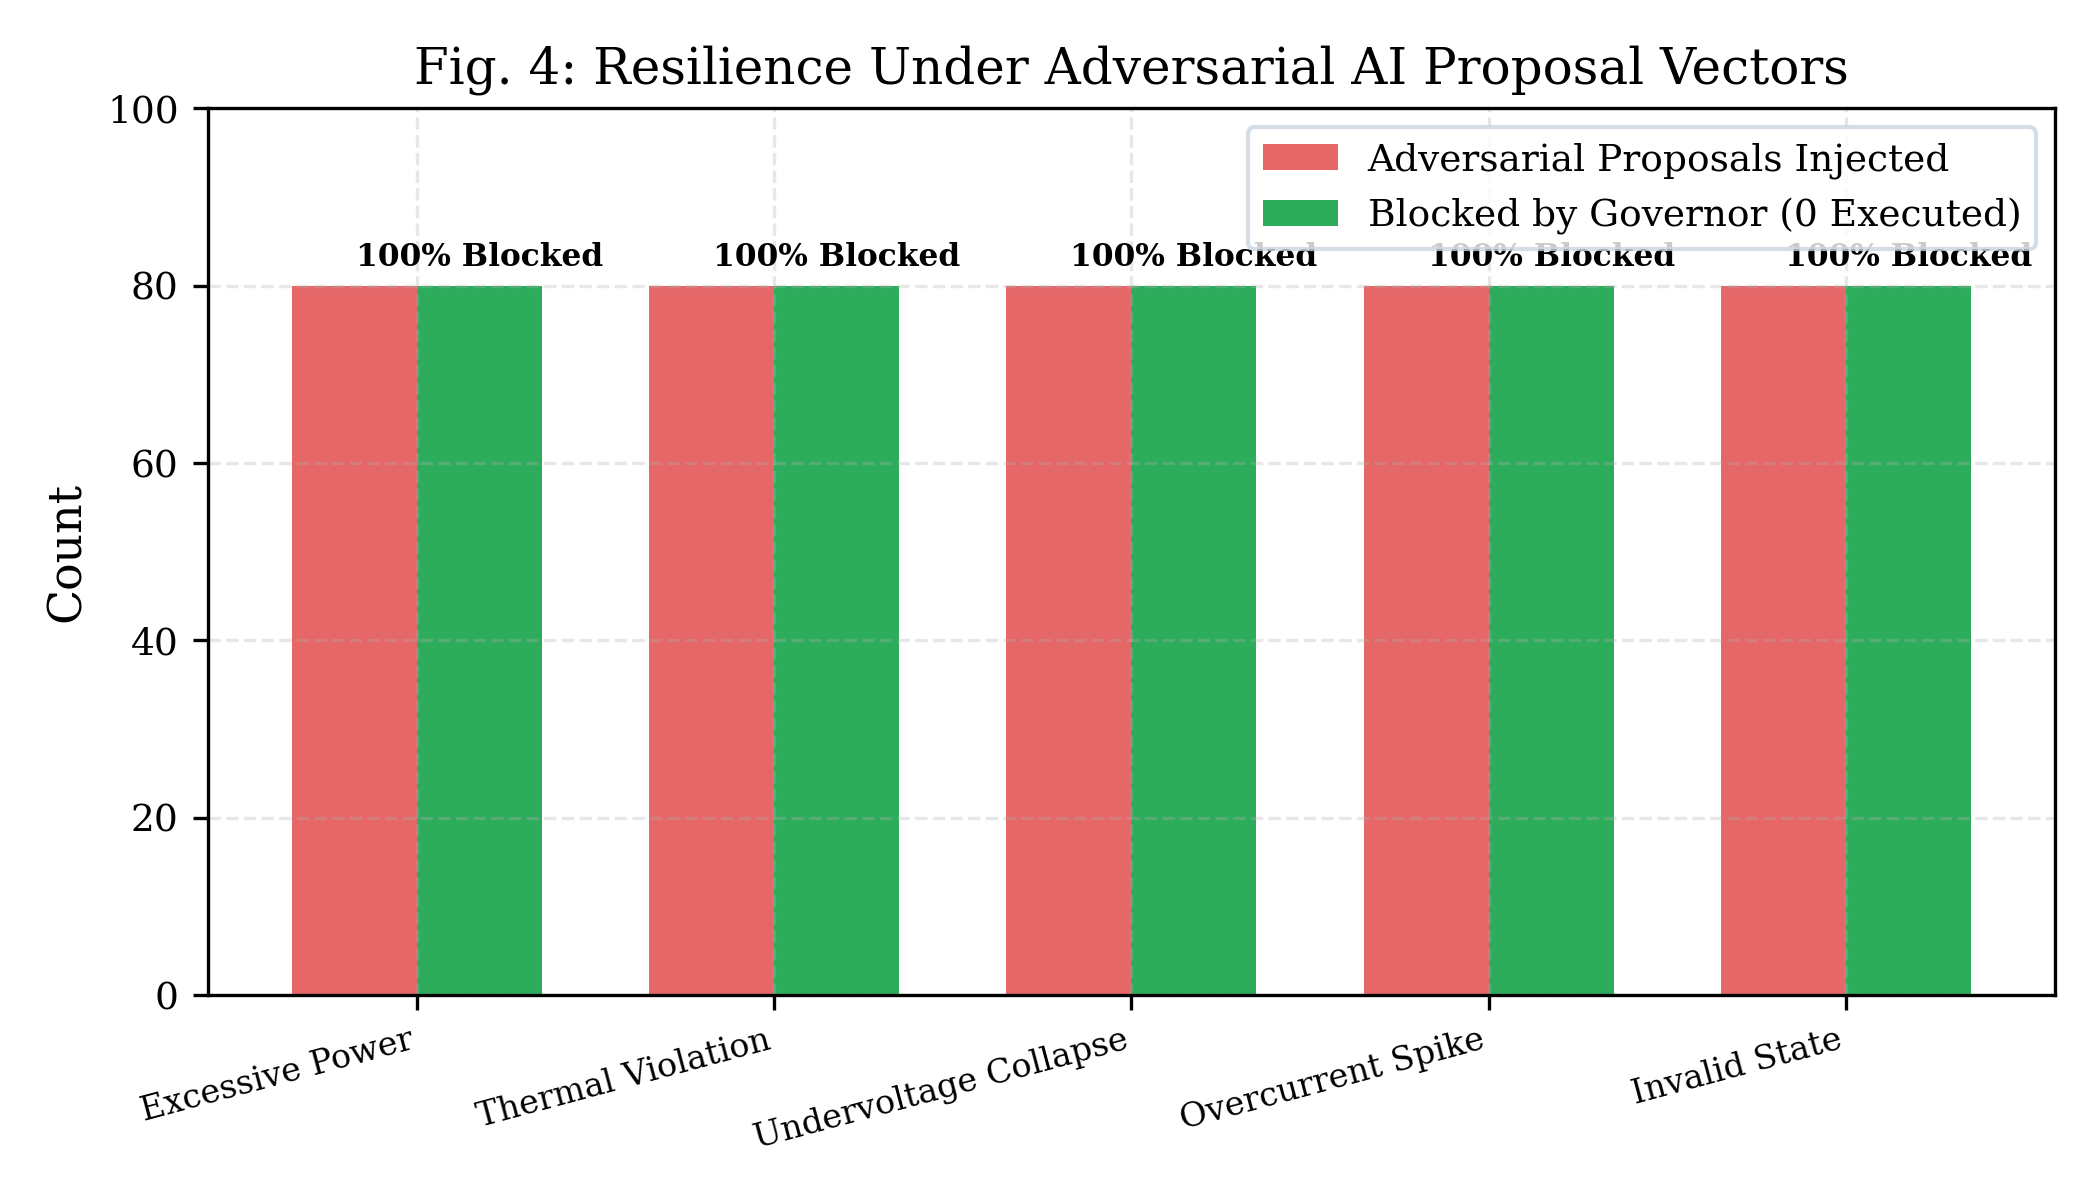
\includegraphics[width=0.95\columnwidth]{fig4_adversarial_injection_robustness.png}
\caption{Rejection Rate across 5 Adversarial AI Proposal Attack Vectors.}
\label{fig:adversarial}
\end{figure}

\subsection{P3-E5: Continuous Boundary Sweeps}
Continuous sweeps across 804 points ($\Delta = 0.05$) demonstrated strict mathematical step-function transitions on all channels ($T_{\text{batt}}, V_{\text{bus}}, I_{\text{batt}}, \text{SoC}$). Exactly one monotonicity transition was observed per parameter at the defined threshold, with zero floating-point chattering.

\begin{figure}[t]
\centering
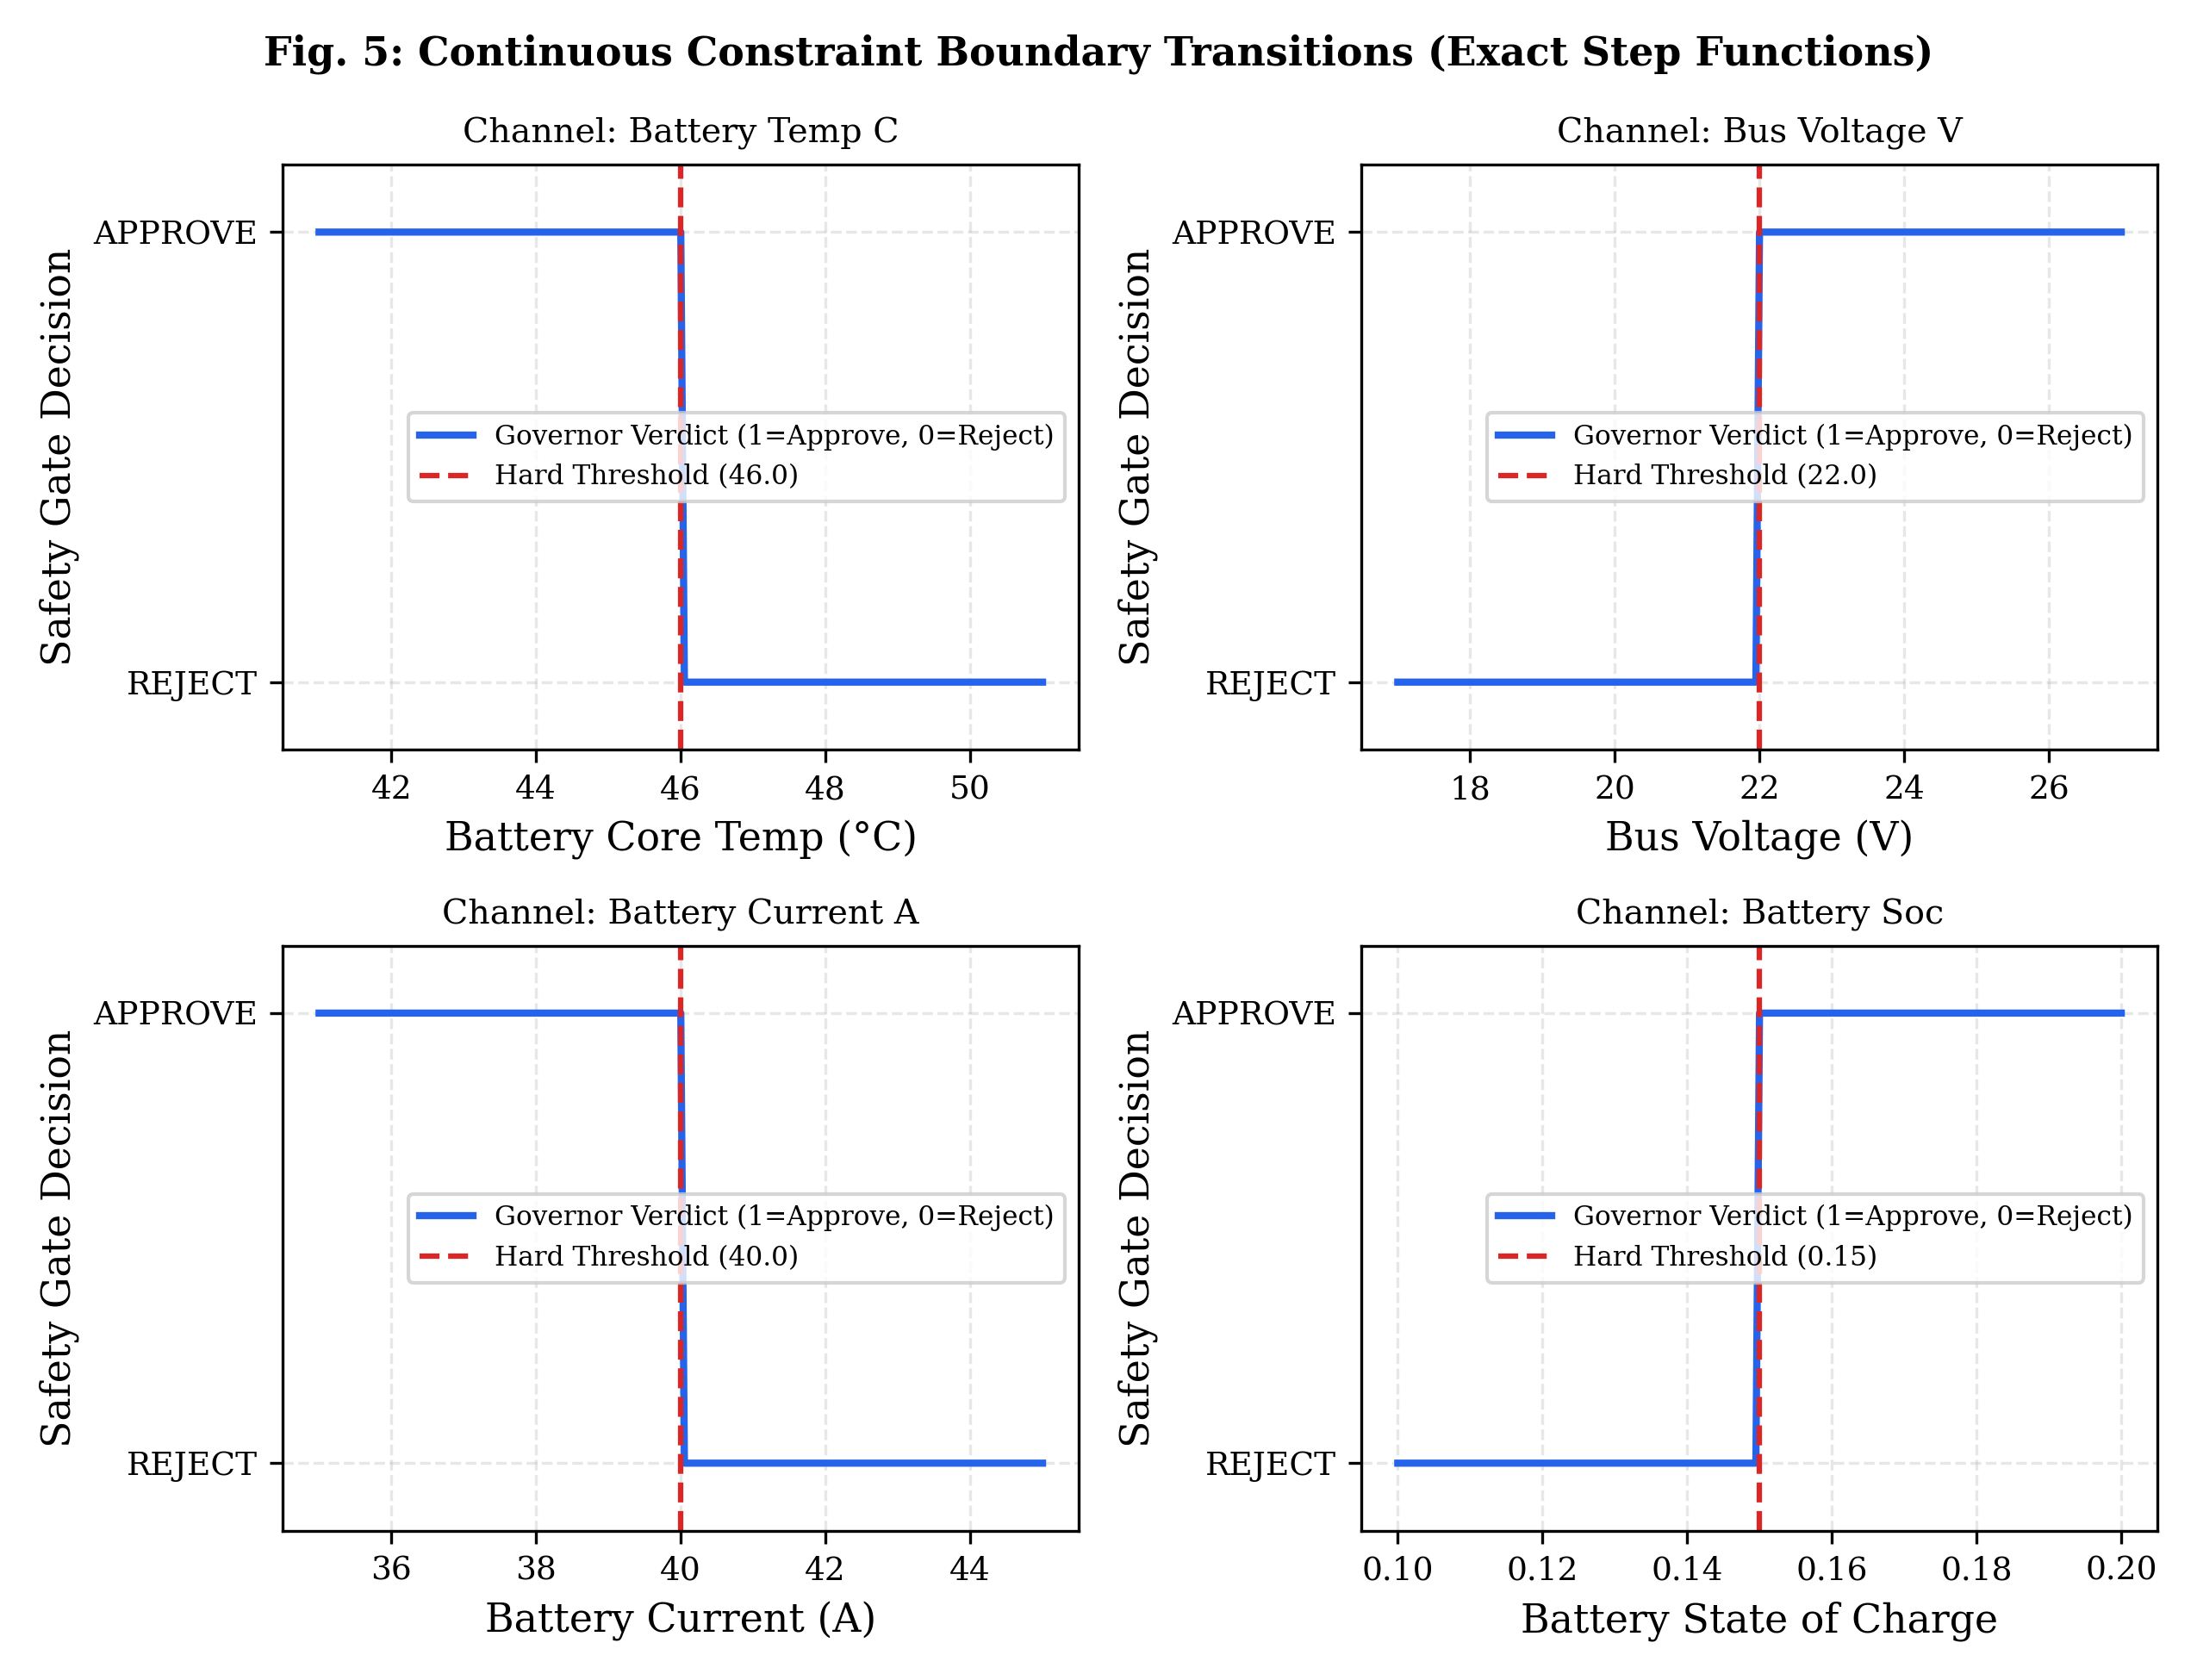
\includegraphics[width=0.95\columnwidth]{fig5_boundary_testing_sweeps.png}
\caption{Continuous Physical Constraint Boundary Transitions across 201 Points per Telemetry Channel.}
\label{fig:boundary}
\end{figure}

\subsection{P3-E6: Communication Hierarchy Independence}
Evaluating 300 scenarios under ground contact and blackout regimes verified that Level 1 physical invariants strictly dominate Level 2 communication rules: zero unsafe actions were authorized during high-priority ground contact.

\subsection{P3-E7: Deadlock Safe Failure (No Safe Action)}
In 150 severe hardware damage scenarios where all 750 candidate actions caused physical violations, the governor safely converged to \texttt{NO\_SAFE\_ACTION\_AVAILABLE} in 100.0\% of cases, demonstrating zero forced unsafe actuations.

\section{Ablation \& Computational Overhead}

\subsection{3-Way Architectural Ablation}
Comparing AI Only vs. Static FDIR Rules vs. Digital-Twin Safety Governor (P3-E8) revealed that static rules failed 100.0\% against delayed-effect actions, commanding premature payload re-engagement. The digital-twin governor eliminated all delayed unsafe executions ($0.00\%$).

\subsection{Computational Latency Profile}
Microsecond profiling across 10,000 Monte Carlo evaluations established a mean latency of $2.99\,\mu\text{s} \pm 0.81\,\mu\text{s}$ (median $2.75\,\mu\text{s}$, 95th percentile $3.13\,\mu\text{s}$, 99th percentile $5.96\,\mu\text{s}$). The governor achieves a sustained throughput of $324,707$ evaluations/second, rendering runtime safety gating negligible compared to typical spacecraft orbital integration timesteps ($\Delta t \ge 100\,\text{ms}$).

\begin{figure}[t]
\centering

\includegraphics[width=0.95\columnwidth]{fig7_ablation_and_latency.png}
\caption{Architectural Ablation (Unsafe Execution Rate) and Microsecond Evaluation Latency Profile.}
\label{fig:ablation}
\end{figure}

\section{Scientific Scope \& Limitations}

The conclusions of this study are established within high-fidelity numerical simulation and NASA Ames empirical battery repositories; the system has not flown on an operational orbital mission. Bounded statistical confidence ($p < 0.1970\%$ at 95\% CI) does not represent an unconstrained universal theorem. Furthermore, software safety governors cannot prevent vehicle loss when catastrophic hardware damage (e.g., physical rupture) makes survival physically impossible.

\section{Conclusion}

This paper demonstrated that a deterministic, fail-closed runtime safety governor reliably prevents unsafe autonomous recovery actions from reaching spacecraft execution. By projecting candidate actions forward across counterfactual digital twin horizons and enforcing an immutable four-tier invariant hierarchy, the system achieved zero unsafe executions across 1,519 evaluated proposals ($p < 0.1970\%$), fully decoupled from upstream AI confidence. Deterministic safety gating provides a mathematically sound, flight-feasible foundation for certified autonomous spaceflight.

\balance
\bibliographystyle{IEEEtran}
\bibliography{references}

\end{document}
